% vim: set ts=2 sw=2 noet spell:

\chapter{Conclusions} \label{chp:conclusions}

\section{Results}

The goal to build a functional demonstrator has been only partially achieved, unfortunately not all of the originally planned features could be implemented. A stable wireless link using QPSK modulation that computes the BER was developed. Because of the issue discussed in section \ref{sec:access-code-issue}, the QAM variant cannot compute the empirical BER.

For both modulation schemes samples from multiple different conditions were collected and analyzed, albeit some assessments could only be conducted when QPSK was used.

\section{Future Work}

\subsection{Improve BER measurements and simulations}

A missing feature in this work is an automated collection of the BER data, which would allow to more easily observe and measure the influence of each parameter in the fading channel model.

\subsection{Improvements in the GUI front-end}

In addition to fixing the issue discussed in section \ref{sec:gui-issue-single-threaded}, a very important feature that is currently missing is the ability to change the fading parameters in real time from within the GUI. Dear PyGUI offers many graphical elements that could be used to control the parameters, however a new GR block would need to be created to propagate the updated values into the flow graph.

\subsection{Portable transmitter on a Raspberry PI}
%TODO : 


\subsection{Channel parameters estimation with PSAM} \label{sec:psam}
%TODO: Picture send mention

An interesting continuation of this work could be to regularly interpolate some so called pilot symbols in the modulated data stream. In short, the pilot symbol assisted modulation (PSAM) technique consists of periodically inserting informationless (known) symbols in the data stream, which can then be used to estimate the fading parameters of the communication channel. More details are presented in \cite{Xiaoyi1999} (and its references) from which the illustrations in \figref{fig:psam} were taken.

\begin{figure}
	\centering
	\includegraphics[width = \linewidth]{figures/xiaoyi-psam-figures}
	\caption{
		Illustration of the pilot symbols assisted modulation (PSAM) frame format (left), and PSAM fading interpolation method (right). The PSAM technique allows to compute the fading (denoted in the figure with \(\tilde{z}_n\)) by interpolating measurements of informationless symbols (pilot symbols) over multiple frames. Both figures were taken from \cite{Xiaoyi1999}, which presents an analytical method to compute the BER from the PSAM and multilevel quadrature amplitude modulation (M-QAM) parameters.
		\label{fig:psam}
	}
\end{figure}

\section{Closing words}

%TODO: 

\section{Acknowledgments}


We would like to thank everyone who took the time to help us. Especially Michel Nyffenegger for his comments. Nicola Ramagnano for his explanations, with the GNU Radio tool. Marcel Kluser, who has provided the equipment. Our friends whose supported us in different ways,e specially Manuel Kritzer and Manuel Spuhler for the correction reading.

%TODO: Prof. Dr. Heinz Mathis for the opportunityto 



